\chapter[Practical work and results]{Practical work and results}
\label{kap:practical_work}

In this chapter,  we will specify the data we are using, provide a biological background for them and describe the way in which they are processed. 
We will describe the practical work and process of creating suitable probes. We will take a look at parameters and specifications we used during the 
run of the Sondovac script. 

\section{Input data}
In this chapter we will take a closer look at the data we are using. We will cover the biological aspect of 
the data. %and compare the data we have to other kinds of data. 
We will also look at how such data is obtained and how it is further processed. 

Sondovac uses a transcriptome, a genome and possibly a chloroplast and mitochondrion. 
We worked with two different sets of input data. These data shared most of the files, differing only in genome. 
%Add some statistics here. #of genes, etc.

The first set used the following data: 

\begin{enumerate}
\item Transcriptome: Alyssum alyssoides
\item Genome: Odontarrhena tortuosa
\item Mitochondrion: Arabidopsis thaliana
\item Chloroplast: Arabidopsis thaliana
\end{enumerate}

The second set used the following data: 

\begin{enumerate}
\item Transcriptome: Alyssum alyssoides
\item Genome: Alyssum gmelinii
\item Mitochondrion: Arabidopsis thaliana
\item Chloroplast: Arabidopsis thaliana
\end{enumerate}

\subsection{Nickel and metallic genes}
We were especially interested in nickel and metallic genes that might be present in these genomes. Therefore, we matched the possible 
probes against nickel and metallic genes and primarily picked those with the greatest similarity. 

%Where do these data come from? Add some statistics
%Maybe move this into the practical part

\subsection{What kind of data we are using}
All the data we are using are from plants, specifically, alyssum alyssoides, alyssum gmelinii, odontarrhena tortuosa and arabidopsis thaliana, 
which are all species of flowering plant from the brassicaceae (mustard) family. This thesis is a part of the process to infer the phylogenetic 
relationship between them. 

%Where does it come from
The hyb-seq protocol allows for lower quality of data, which means that dried plants from herbarium can and were be used. The genetic data was obtained from 
another company after sending them the basic plant material. 
%TODO bližšie popísať podľa odpovede

The nickel and metallic genes are from the web page https://www.arabidopsis.org/tools/bulk/sequences/. The used dataset was AGI transcripts and AGI coding sequences. 
It was searched against sequences for all gene models/splice forms. 

\section{Autometed selection of probes}

%Definition of the problem goes here
When making probes, we usually want to get exact number of bases, because the created probes are later passed to another 
company, such as MYcroarray (USA) \cite{mycroarray} that will create the actual physical probes from them. These companies 
usually charge for processing of a precise number of bases. To save money, it is best to fill this number to the brim. 
Therefore, when we have several sequences available, we want to select such sequences, that the sum of thei lenghts makes the 
highest number possible, but does not exceed the given limit, let us say $1,000,000$ of base pairs. 

Aside from this, we often have other requirements on the selected sequences, usually based on biological evidence. There might be 
sequences we do not want in our selection, or even sequences we might want to add. 

This selection is usually done by hand or a series of programmes. It would be beneficial, if this part too, was automated. 

We want to create a script, that would work with the second part of sondovac and would be able to select the best possible 
sequences to fill up the limit. This script would take into account any sequences we want to keep, or those we do not want in 
the result. 

We need specific genes - responsible for nickel and metal binding. If these genes are present among our sequences, they have 
to be in the result. We will take the largest possible output file from sondovac\_part\_b: the one with the lowest minimum total locus length. 
From this file, we will select the required genes. Any additional probes will be chosen by a combination of greedy algorithm and a knapsack. 


\section{Process overview}
After several tries, it was estabilished that we will make probes from two sets of data to cover broader spectrum of plants they can 
be used for. We ran the Sondovac script for each set and got two resulting sets of possible probes. From these possible probes, we 
proceeded to pick those that fit the criteria the best. Consecutively, the probes have to make up to $1,000,000$ base pairs, due to 
restrictions of the probe-making company. 
To pick suitable probes, we matched each data set to nickel and metal genes and chose those that aligned with them. We matched the 
data sets against each other and picked probes by similarity. We chose only one of the probes that matched. The other one 
wasn't included in the final probes to avoid duplicates. Finally, the rest was picked so they would make up the $1,000,000$ bases to 
make the most of the space. 


\begin{figure}
\centerline{
	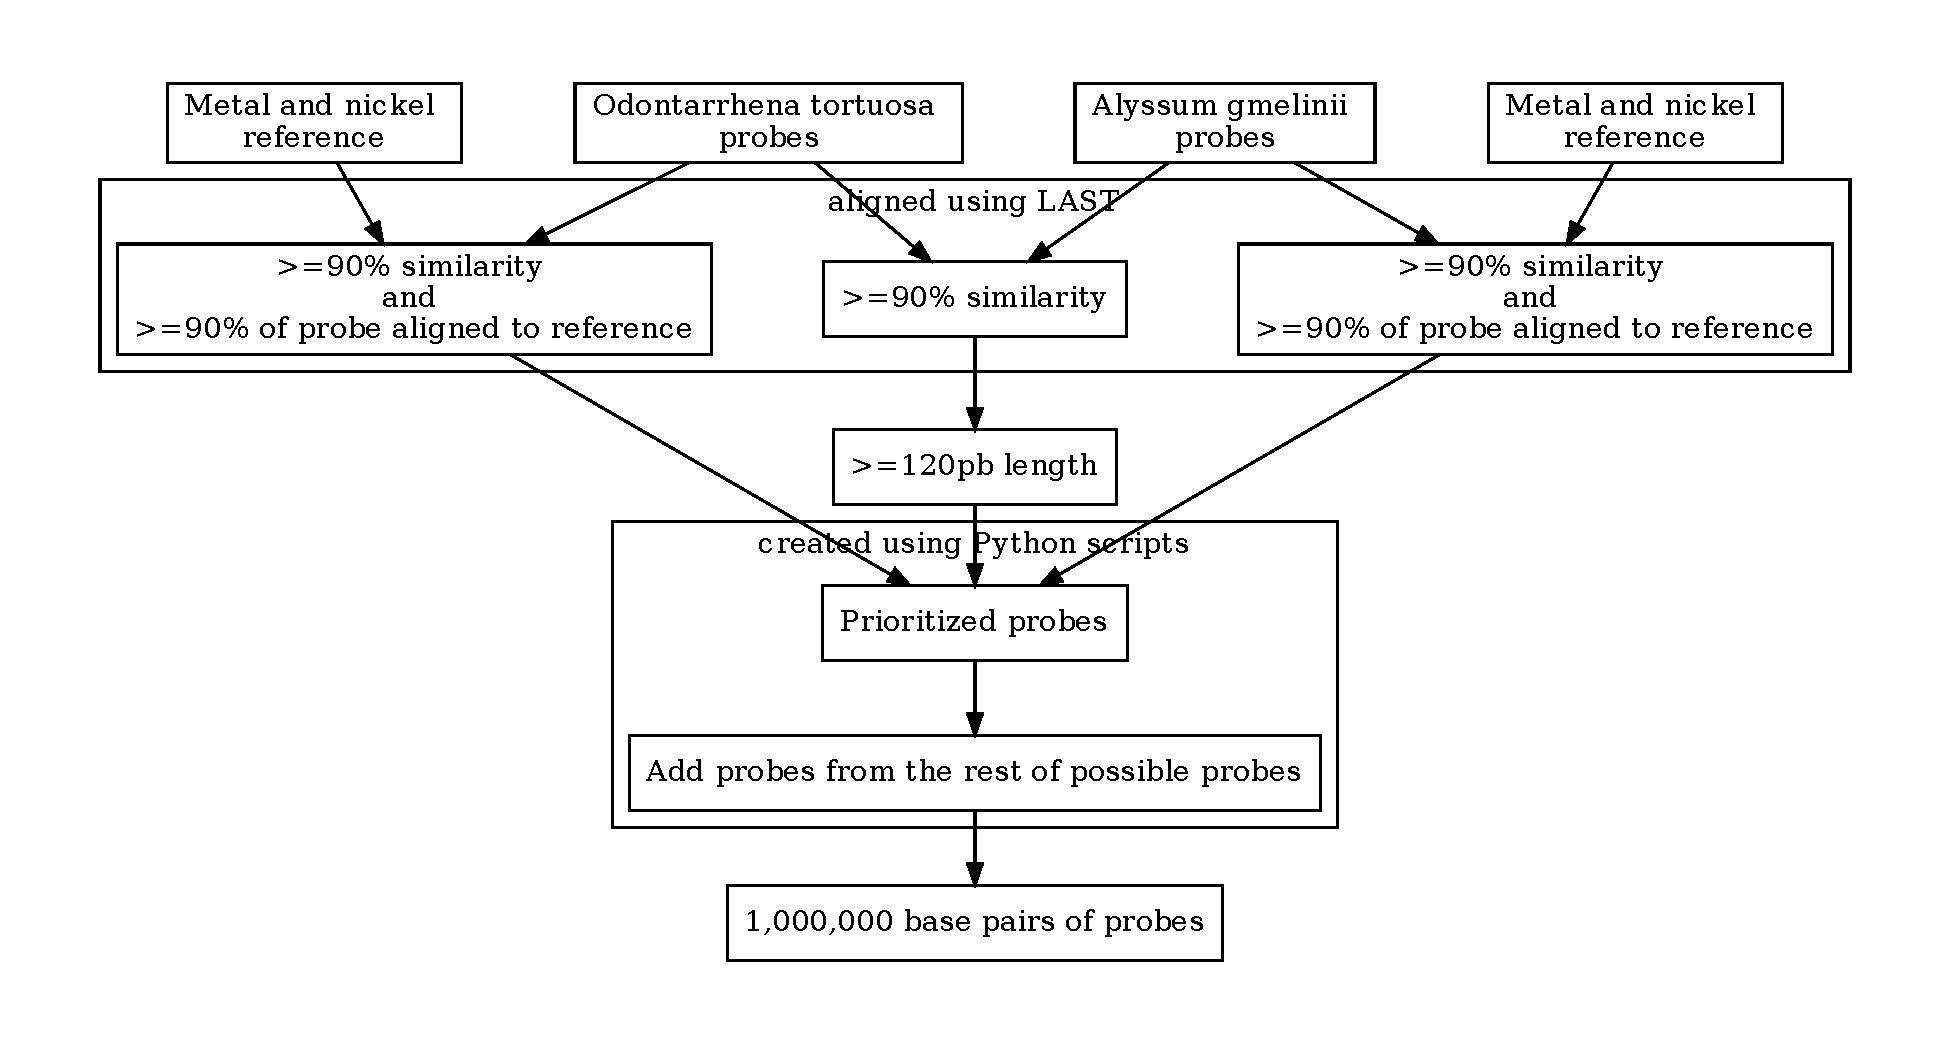
\includegraphics[width=1\textwidth]{graphs/selecting_probes}
}
\caption[Workflow of picking the probes]{Flowchart illustrating the workflow of picking the final probes from all possible probes.}
\label{obr:picking_probes}
\end{figure}



\section{Using the pipeline}
The possible probes were produced by running the script Sondovac on two different data sets. We then picked suitable probes from 
the resulting probes. 

%Sondovac parameters
We set the minimal total locus length on $360$ for both datasets - the least possible minimal total locus length - so we could get 
the largest amount of possible probes to pick from. 

%add some statistics about created probes


\section{Probe picker}
Probe picker is a script that we coded to help with picking the final probes. It is coded in python. The probe picker requires 
a list of all possible probes to pick from as an input. It can be also given a list of probes we definitely want in the result - such as the 
ones that aligned with the nickel or metallic genes or intersection of the two genomes - and a list of probes we do not want in 
the result - such as duplicates or sequences that are too similar to each other, for 
example the second of the pair of aligned genes from the two genomes we had. 

Aside from lists of probes, the Probe Picker requires a target number of bases to be set and a threshold after which the program should 
change approaches. After reaching this threshold, the program will start picking the probes so they make up to the $1,000,000$ bases instead of 
taking probes in order. 

%Describe the workflow
%Matching name_sequence & length_name
After the input files are obtained, the Probe Picker will match a sequence's name to sequence using dictionary data type and the sequence's length to 
its name using an array. 

Then, the script puts sequences to keep and sequences to remove into a dictionary, creating a set for each data. 
Finally, the actual selection ensues. 
First, the probe is picked if it isn't in the sequences to remove. If it's also in the sequences to keep, it is automatically put into the output. 
If the sequence isn't amongst the sequences to remove and it isn't amongst the sequences to keep either, it's saved for later processing; for when we are 
picking sequences in order or picking them so they make up to the target number of bases. 

After picking the sequences that are present in the list of sequencest to keep, we start filling the rest of the space by the remaining sequences. We sort the 
sequences in descending order and pick the largest ones until we hit the threshold. The larger the sequence, the higher the possibility that it's relevant 
when it matches with something. 

After reaching the threshold, we switch to using dynamic programming to make up to the target number of bases with best possible accuracy while not exceeding this 
number. 

\begin{figure}
\centerline{
	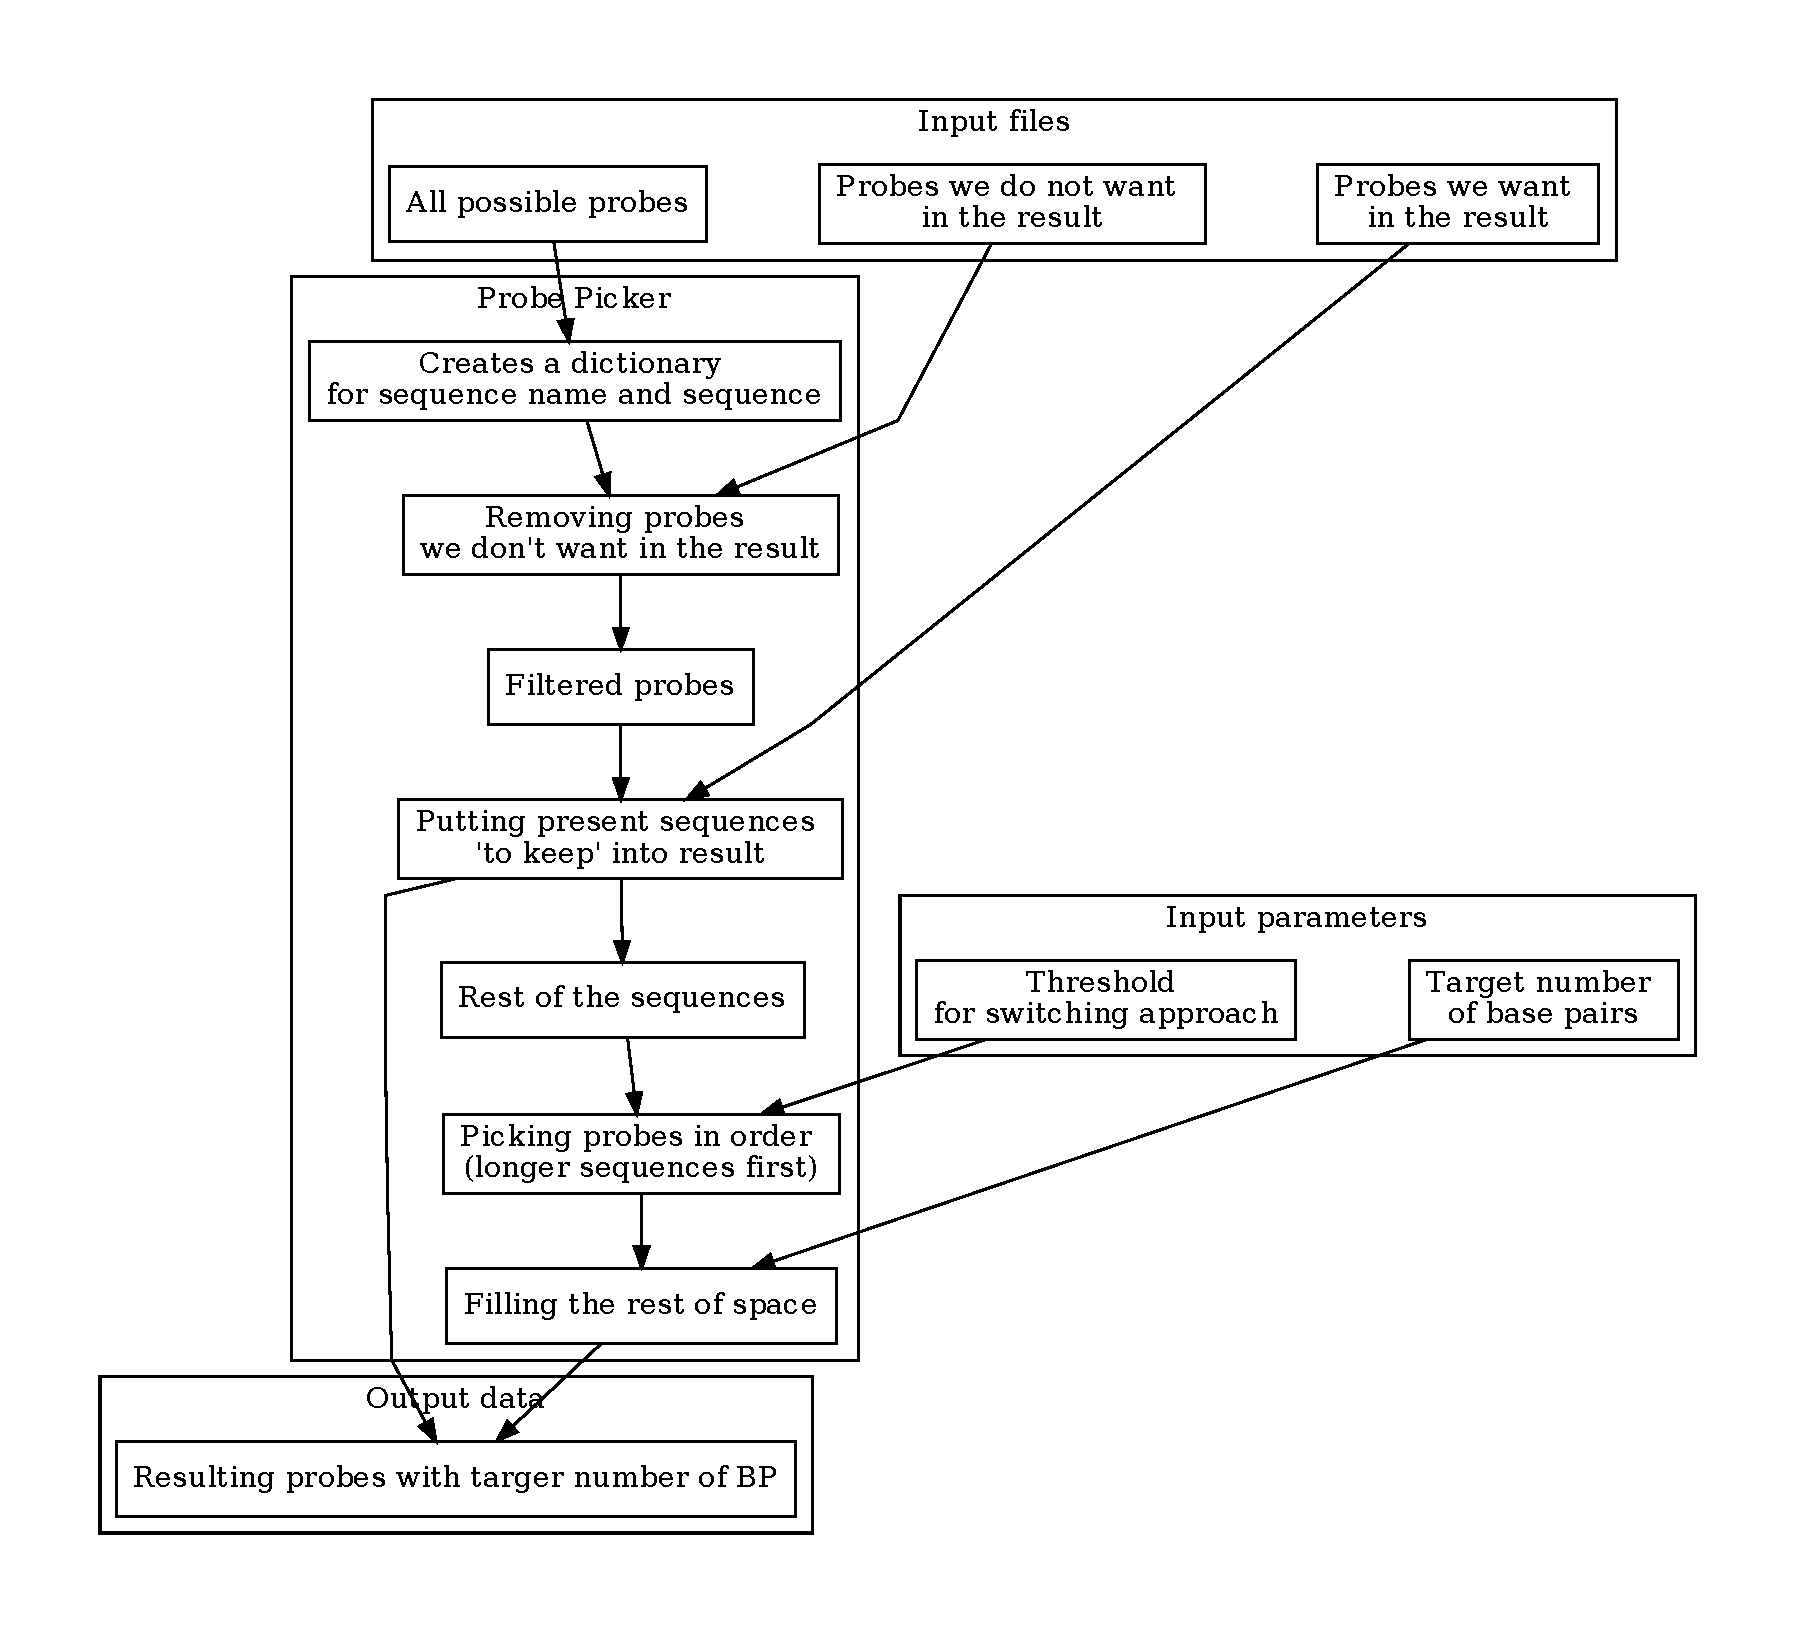
\includegraphics[width=1\textwidth]{graphs/probe_picker_workflow}
}
\caption[Workflow of Probe Picker script]{Flowchart illustrating the workflow of the script "Probe Picker".}
\label{obr:probe_picker}
\end{figure}


\subsection{Knapsack problem and dynamic programming}
%Write about knapsack problem
The knapsack problem is a well known problem in combinatorial optimalisation. The problem goes as follows: If we are given a knapsack with a weight limit and a 
set of items where each has a value and weight, what is the biggest possible value we can pack into the knapsack while the total weight of items is less or equal to 
the knapsack's limit. 
%How does this apply to our problem
The Probe Picker presents us with a problem, where we have $n$ numbers to choose from and a limit $l$ that we mustn't overstep. This is a variation of the knapsack problem, 
where the value of each item is equal to its length, or rather, the number of bases it consists of. As a result, we want a list of bases that make the most of the possible space; 
we want to fill the "knapsack" as precisely as possible without overstepping the limit. 
%Definition of informatic problem
The original version of 
%Theory, solution, and stuff. Why we can make it quick by dynamic programming


\subsection{Picking the genes to keep and remove}

We decided to keep probes, that align with nickel and metal genes and also reads that are present -- or at least have certain similarity -- in the intersection of both 
Odontarrhena tortuosa and Alyssum gmelinii genome. Naturally, we also want to create a list of probes to remove, where we would put the probes that are too similar to each other, in this 
case the second of the aligned reads from the intersection of the genomes. 

First step was to align probes with metal and nickel reference. We used LAST -- a software for finding similar regions between sequences and aligning them. \cite{last} 
We used the basic settings of LAST and the commands "lastdb" to create a database from reference metal and nickel sequences. After that, we used the command "lastal" to 
align the probes to the reference. 

Both the odontarrhena tortuosa probes and the alyssum gmelinii probes wer were aligned to both metal and nickel reference, resulting in four different alignments. 

After this, we aligned the odontarrhena tortuosa probes to the alyssum gmelinii probes, as we wanted an intersection of these probes. 

These lists are then filtered using a Python script to pick those, that meet the requirements. 
In the case of the probes aligned with metal and nickel reference, it was required for at least 90\% of the probe to fit into the reference sequence and this part had to have at least 90\% similarity. 
The Python script determined the similarity based on ration of achieved score and the maximal possible score. If at least 90\% of the probe fit into the reference was determined on ration of the alignment lenght 
and probe length. 
Another Python script was created to filter the aligned Odontarrhena tortuosa and Alyssum gmelinii genome probes. In this case, the requirements were that the similarity had to be at least 90\% and the length of the probe had to be at least 120 bp. Later, the requirement on similarity was changed to $\geq$ 80\% due to low number of aligned probes. 

We coded additional script that creates the list of probes we want to have in the result and those we want to remove from these aligned sequences. 
This script takes the list of names of aligned probes that meet the requirements -- the output from the previous script -- and a list of probes that aligned to the metal and nickel reference (or probes to probes in case of alignment of Odontarrhena tortuosa and Alyssum gmelinii probes) and creates a list of probes to keep from this file. It then sorts the list of aligned probes and sorts them based on similarity, so the 
probes with best score are the ones that are taken first. 

The script takes probes from this list in order and for each probe, it puts this probe (both sequence and name) into the final list of probes we want to keep. Then it puts the probe it aligned with or any other 
similar probes and puts these into the list of probes we want to remove. This is done to avoid having duplicates or sequences that are too similar to each other amongst the probes. If 
